\chapter{Role in Overall ModelDB System}
ModelDB S+C was not built in isolation. It interacts with a number of other
systems in an overall system called ModelDB \cite{hilda}. ModelDB is a system for machine learning
model management. It includes:

\begin{enumerate}
\item a web application for visualizing and examining data about models and operations
\item a client, like the Spark Client, designed for Python's Scikit-learn machine learning
library
\item a command line toolkit that includes a versioning system for code
\item a prediction store for the predictions made by models
\end{enumerate}

Figure \ref{fig:system_architecture} showed the system architecture
of ModelDB S+C. Figure \ref{fig:full_system_architecture} augments Figure \ref{fig:system_architecture}
to show how some of the other pieces of ModelDB interact with ModelDB S+C. The prediction store
is excluded from the figure because it currently has not been integrated into the rest of the ModelDB
system.

\begin{figure}
  \centering
  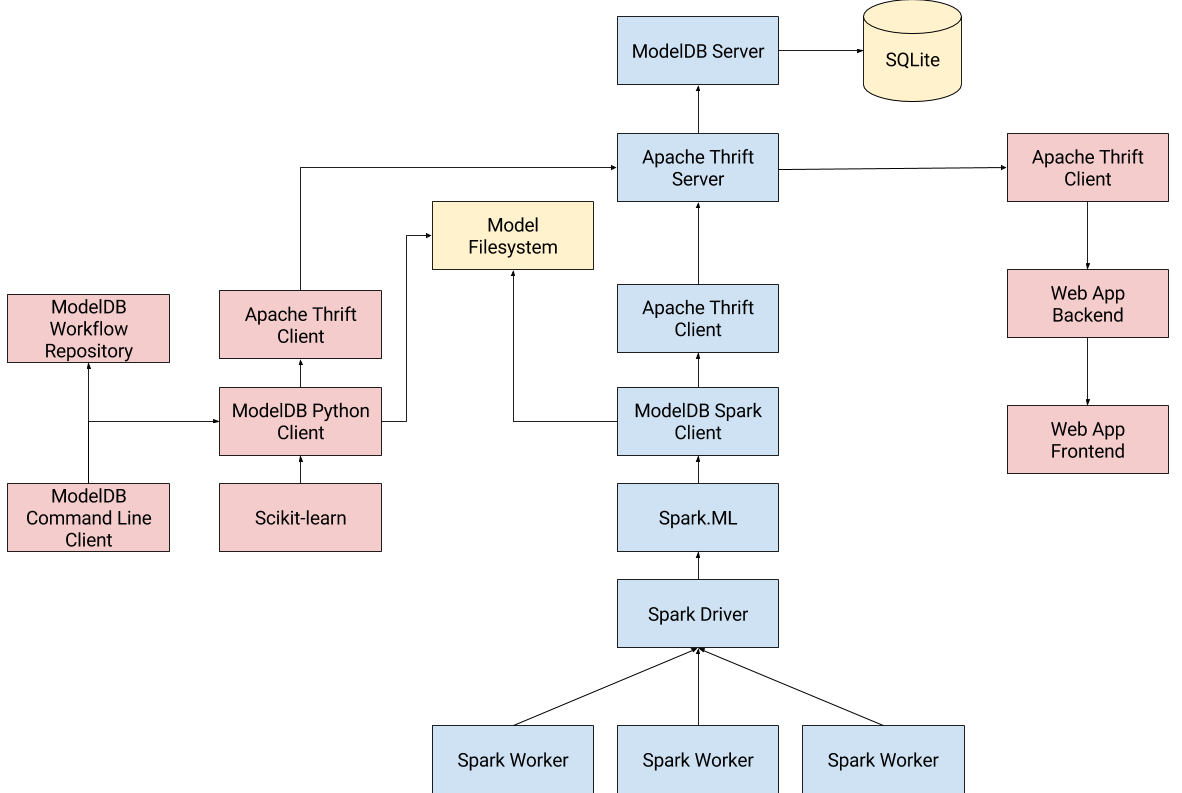
\includegraphics[height=4.0in]{full_system_architecture}
  \caption{
    The overall architecture of ModelDB that shows the components
    that interact with ModelDB S+C. The arrows indicates the flow
    of operations + models data. 
  }
  \label{fig:full_system_architecture}
\end{figure}

The other systems in ModelDB can be seen as use cases that demonstrate how ModelDB S+C
can serve as a foundation for other applications.

\section{Scikit-learn Client}
ModelDB includes a client for Python's Scikit-learn machine learning library. Like the
ModelDB Spark Client, the Scikit-learn Client also utilizes the ModelDB Syncer abstraction,
the Syncable Event abstraction, and the "Sync" API (e.g. fitSync, transformSync). This Scikit-learn
Client was inspired by the abstractions in ModelDB Spark Client, and demonstrates that the ModelDB Server
abstractions (e.g. FitEvent, TransformerSpec) can generalize to other machine learning libraries and that
ModelDB Spark Client abstractions (e.g. ModelDBSyncer) can also generalize to other machine learning libraries.

\section{Command Line Toolkit}
ModelDB includes a command line toolkit that allows users to record various operations (e.g.
evaluation of a model) without using any kind of machine learning library. This command line toolkit still
uses the underlying abstractions in ModelDB Server, showing that they can generalize even if there is no machine learning
library.

\section{Web Application}
ModelDB includes a web application that can display information about models and visualizations of
the model building process. This web application is built directly on the API methods exposed by the ModelDB Server,
and does not actually use the database directly. This shows how an application can be built on top of ModelDB Server's 
data and API.

\section{Possible Database Applications}
Although no applications in ModelDB access the database directly, the database, on its own, 
could serve as a building block for other applications. Additionally, the database could simply be used in other data management
systems, like DataHub \cite{datahub}.
